\chapter{序論}
現在,機械学習の分野ではディープラーニングが盛んに研究され,とくに時系列データを扱うためには各ノードが次の層への結合のみを持つ順伝搬型(feed-forword)ではなく以前の層への結合も持つリカレントニューラルネット(RNN)と呼ばれる方式が使われている.しかし,一般のディープラーニングにおいて,現実的な精度を得るためには多くの隠れ層を必要とするがその学習は必ずしも現実的な計算量では終わらない.これは多数の隠れ層を持つニューラルネットワークでは,ノード間の結合が非線形な活性化関数で定義されるため,教師データに対する数値解析的なフィッティングしかできないことに起因する.そこで,学習効率を上げる方法としてRNNを物理現象によって再現したリザバが登場した.\par
このリザバからの複数の出力の積和演算をすることで特徴量を抽出することができる.特に,学習するのはリザバではなく積和演算の重みのみであるため学習コストを低減させることができる.光で入出力を行うフォトニックリザバにおいては高速な画像認識に用いることができる可能性が報告されている.しかしながら,現状では出力を光のまま積和演算することは難しいためフォトダイオードによって電気に変換し積和演算・並びに学習を行うことが検討されている.ここで,積和演算が画像認識速度のボトルネックにならないよう高速な処理が必要なため,アナログ信号の積和演算を行うギルバート乗算回路を使用することが本学で検討されていた.フォトニックリザバに用いる後処理部は図\ref{fig:1_config}に示すように,リザバからの光出力をフォトダイオード(PD)で電気に変換し,乗算器を用いて制御電圧による重みづけを行う.重みづけされた各信号を単一の抵抗(Load)に流すことで和をとる.この乗算器の部分についてギルバート乗算回路を用いることを検討していた.この構成では各乗算器の出力が共通になっているため,出力は合計の出力範囲は単一の乗算回路の出力範囲と変わらず,リザバからの出力が増えるだけ各信号の入出力範囲の制限が大きくなるため出力振幅が小さくなることで信号対雑音比(S/N比)の劣化が懸念される.
\begin{figure}
        \begin{center}
        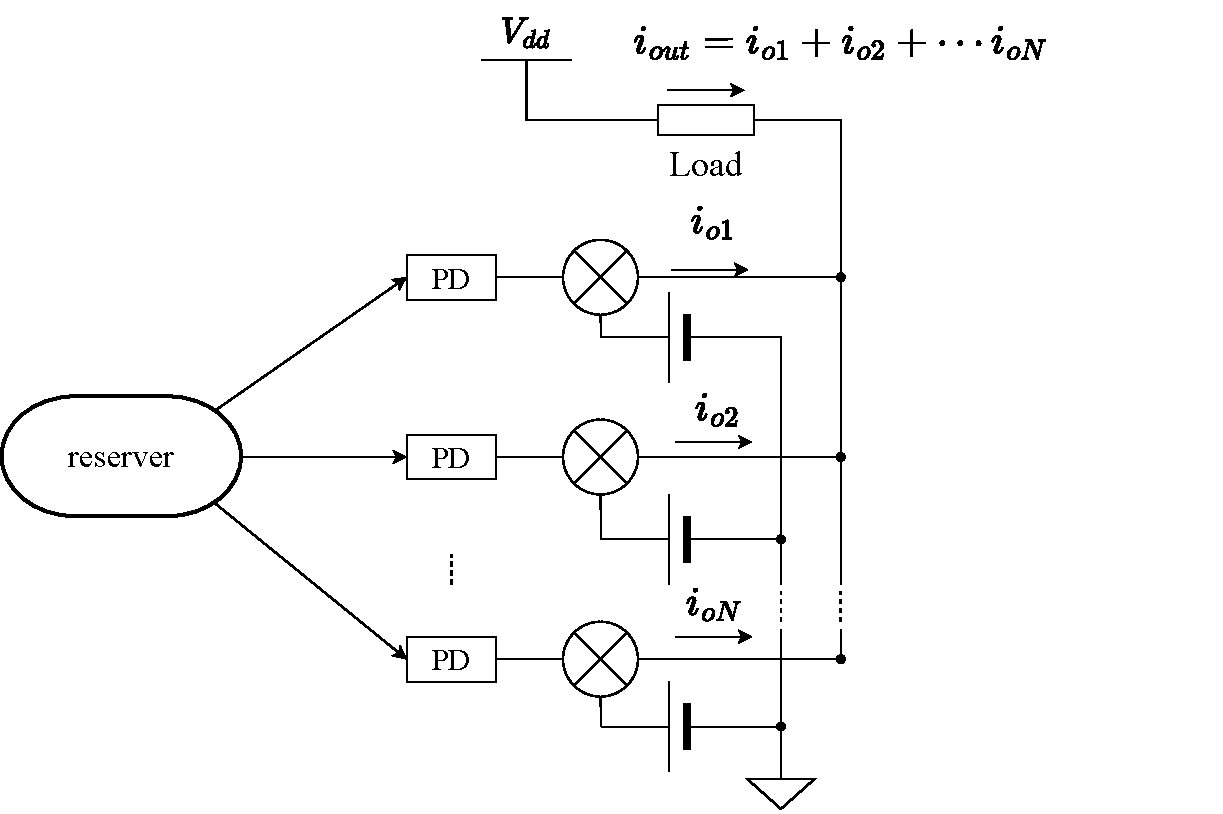
\includegraphics[width=0.99\textwidth]{figures/chapter1/config.pdf}
        \caption{フォトニックリザバの後処理部の構成}
        \label{fig:1_config}
    \end{center}
\end{figure}
\par
本研究では,S/N比向上のため乗算回路単体の出力振幅を拡大する構成を提案する.本論の構成は以下のとおりである.まず2章で検討していたギルバート乗算回路構成を示し,小信号解析を行うことでその特性を確認する.さらにMOSFETが遮断しない条件を用いて出力範囲を導出する.3章において提案する回路構成についての基本的な方針を示し,小信号解析において提案回路がギルバート乗算回路同様,アナログ信号の乗算が可能であることを明らかにする.また,その出力範囲を導出しギルバート乗算回路に対し出力範囲を広げられることを示し,シミュレーション上でも確認する.最後に,4章で結論並びに今後の展望について述べる.